\section{Introdução}
Este trabalho prático consiste numa aplicação web que implementa um repositório digital de obras musicais e respetivas partituras, respeitando a estrutura do modelo de referência internacional \textbf{OAIS} (\textit{"Open Archive Information System"}).

Neste modelo existem 3 tipos de atores: o utilizador do tipo \textbf{produtor} que deposita partituras e cataloga as obras, o \textbf{administrador} que gere e mantem o sistema e, por fim, o \textbf{consumidor} que consulta e descarrega a informação disponibilizada. Assim, segue que cada um pertencerá a um de três tipos de utilizadores do sistema, com permissões específicas à sua posição segundo o modelo \textit{OAIS}.

\begin{figure}[H]
\begin{center}
    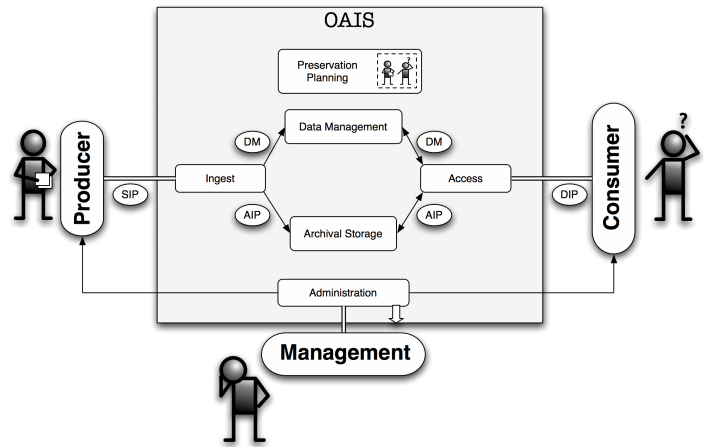
\includegraphics[width = 0.6\textwidth, keepaspectratio]{imgs/OAIS.png}
    \caption{Estrutura base de um repositório do modelo \textit{OAIS}.}
    \label{fig:oais}
\end{center}
\end{figure}

Relativamente à estrutura da aplicação, segue o modelo \textbf{MVC} (\textit{Model-View-Controller}), sendo que a base de dados utilizada foi o \textit{MongoDB}.

\begin{figure}[H]
\begin{center}
    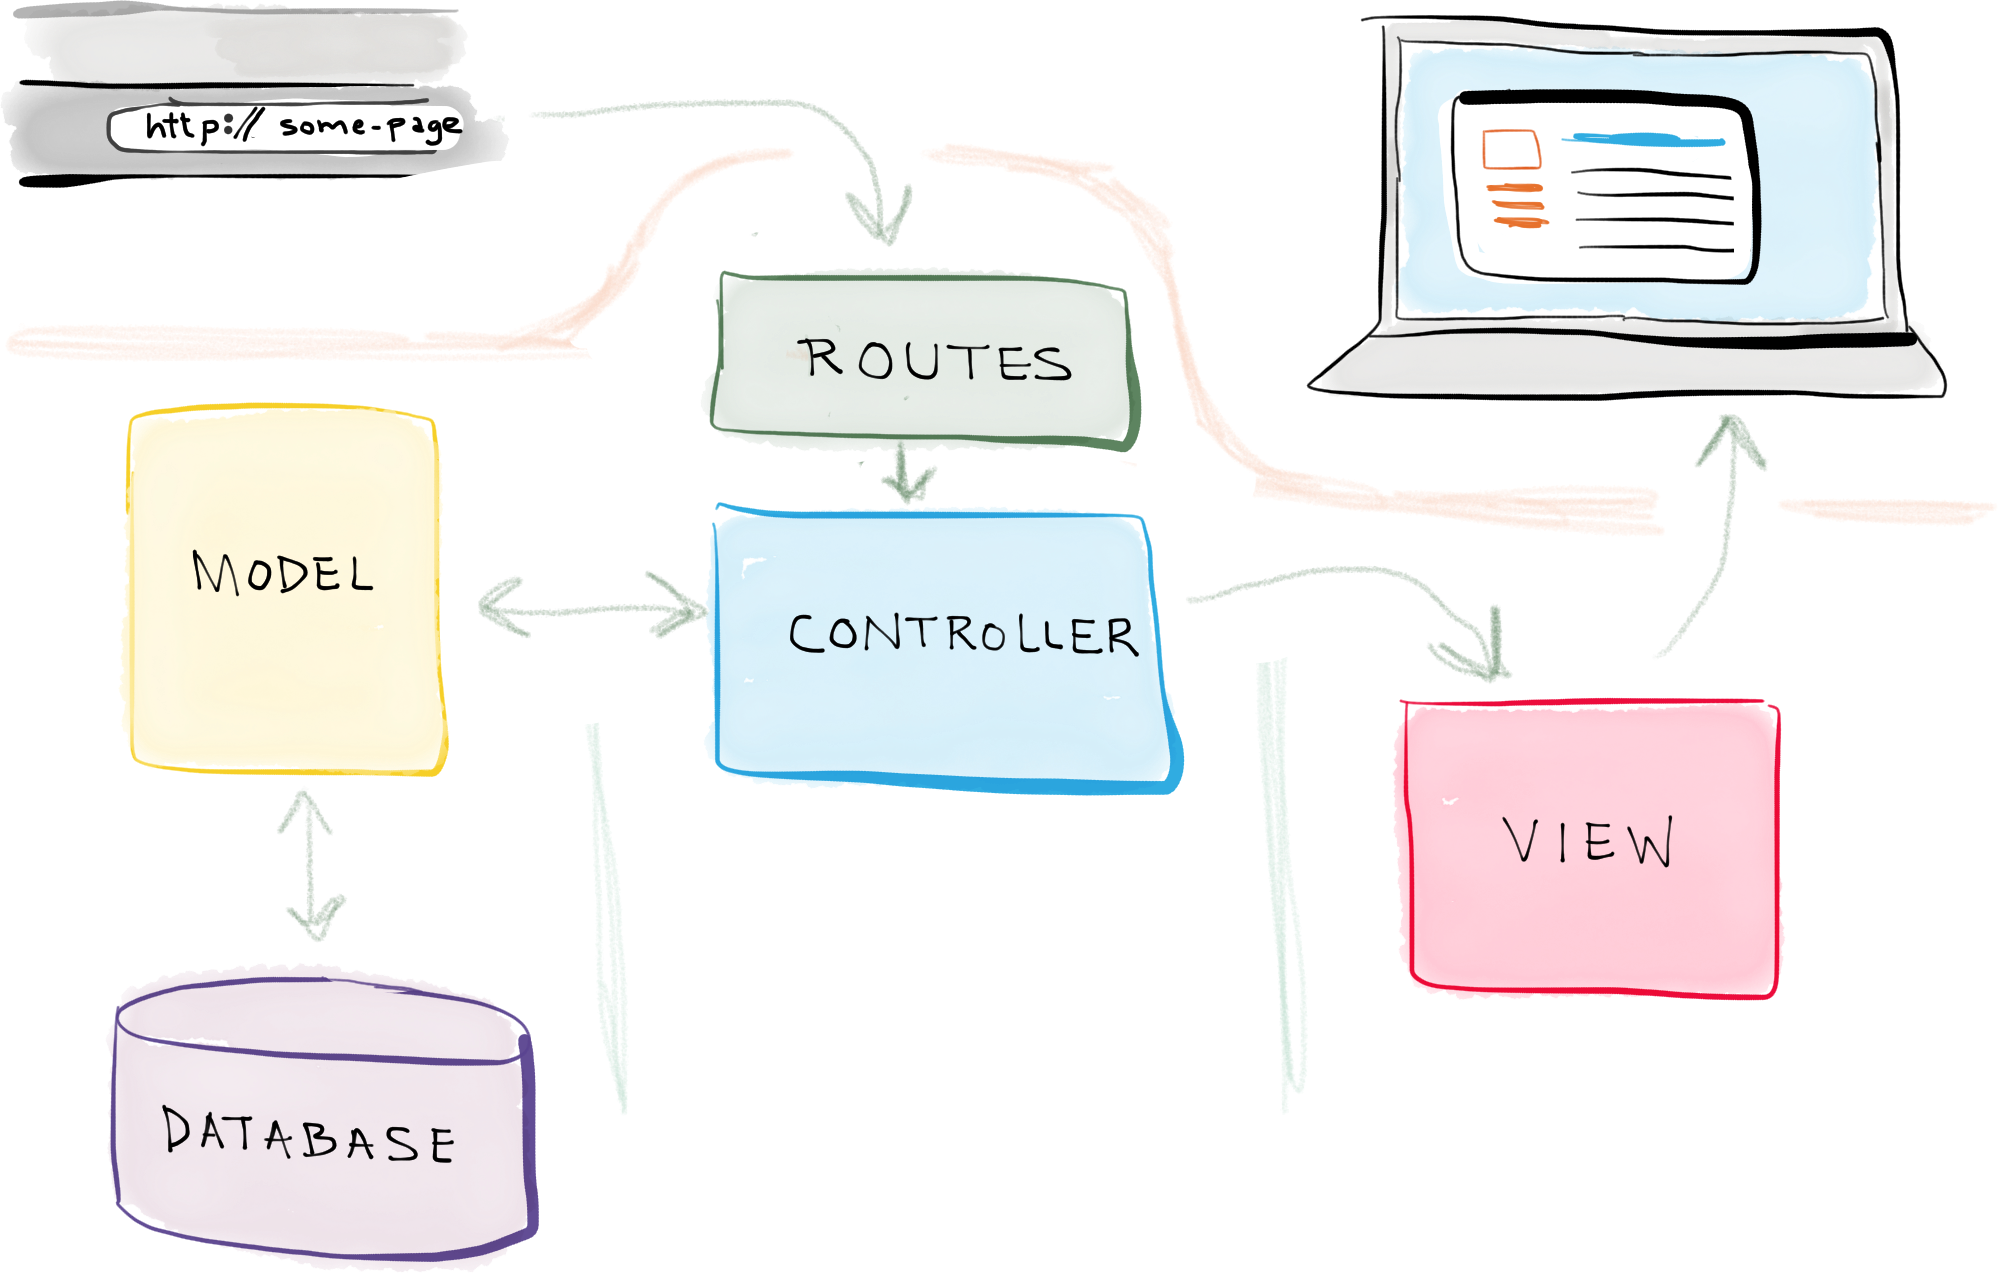
\includegraphics[width = 0.6\textwidth, keepaspectratio]{imgs/mvc.png}
    \caption{Estrutura base da aplicação}
    \label{fig:mvc}
\end{center}
\end{figure}